\section{Raytracing}

\subsection{Farbwahrnehmung und Farbmodelle}
\subsection{Globale Beleuchtungsmodelle und Rendergleichung}
\subsubsection{BRDF und Reflectancegleichung }
Die sogenannte bidirektionale Reflektanzverteilungsfunktion (engl. Bidirectional Reflectance Distribution Function, BRDF)
ist eine Funktion $f_r (x, \omega_i, \omega_r)$, die das Reflexionsverhalten der Oberfläche eines Materials beschreibt. 
Sie hat als Eingabe die ausgehende Richtung $\omega_r$ und die eingehende Richtung  $\omega_i$ am Punkt $x$. 
Sie  liefert den Quotienten aus Strahlungsdichte und Bestrahlungsstärke für die ausgehende Richtung $\omega_r$ und die eingehende Richtung  $\omega_i$ am Punkt $x$.
Sie lässt sich für Materialien experimentell mit Hilfe von Sensoren gewinnen. 

 \begin{figure}[H]
    \centering
    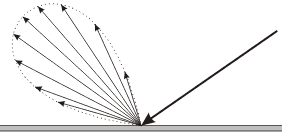
\includegraphics[width=0.6\textwidth]{images/brdf2.png}
    \caption{BRDF Funktion}
    \label{fig:raytracin_brdf}
\end{figure}

\begin{align*}
L(x, \omega_r) = \int_{S^2}f_r (x, \omega_i, \omega_r) \cdot L(x, \omega_i) \cdot <\omega_i, n> d\omega_i
\end{align*}
 
\subsubsection{Die Rendergleichung}

\subsection{Raycasting}
\subsubsection{"Klassisches" Raytracing}
\subsubsection{Monte Carlo Integration und Pathtracing}
\subsubsection{Datenstrukturen für Bereichsabfragen}

\subsection{Raymarching}
\subsection{Labor}
\subsubsection{Blender}
\subsubsection{Echtzeitfähiges Raymarching in WebGL}
